%
%\appendix
%\setcounter{chapter}{3}
%\renewcommand{\thechapter}{\Alph{chapter}}
%
%\begin{figure}[ht]
%	\begin{center}
%		\begin{tikzpicture}[scale=1.2]
%		\SetVertexSimple[Shape=circle,MinSize=5 pt,FillColor=white]
%		\Vertex[x=0.00, y=0]{0}
%		\Vertex[x=0.00, y=2.00]{1}
%		\Vertex[x=1.90, y=0.62]{2}
%		\Vertex[x=1.18, y=-1.62]{3}
%		\Vertex[x=-1.18, y=-1.62]{4}
%		\Vertex[x=-1.90, y=0.62]{5}
%		\Edges(1,2,3,4,5,1)
%		\Edges(5,0,c,2)
%		\Edges(0,e,3)
%		\Edges(0,c)
%		\Vertex[x=0.59, y=0.19]{c}
%		\Vertex[x=0.36, y=-0.49]{e}
%		\tikzstyle{edge} = [draw,line width=2.5pt]
%		\draw[edge] (5) -- (1) -- (2);
%		\draw[edge] (1) -- (0) -- (e) -- (c) -- (e) -- (3) -- (4);
%		\tikzstyle{edge} = [draw,line width=1pt]
%		\draw[edge] (0) -- (c);
%		\draw (0,2.3) node {$a$};
%		\draw (-2.2, 0.62) node {$b$};
%		\draw (2.2, 0.62) node {$e$};
%		\draw (-0.2, -0.2) node {$c$};
%		\draw (0.59, 0.5) node {$d$};
%		\draw (0.66, -0.49) node {$f$};
%		\draw (-1.48, -1.62) node {$g$};
%		\draw (1.48, -1.62) node {$h$};
%		\end{tikzpicture}
%	\end{center}
%	\caption{Un grafo y uno de sus árboles expandidos} \label{f6.3}
%\end{figure}
%\chapter{Grafos planares}

\appendix
\setcounter{chapter}{3}
\renewcommand{\thechapter}{\Alph{chapter}}
\chapter[Grafos planares]{Grafos planares}

\begin{section}{Grafos planares}\label{Ap4.1}
Usualmente el diagrama de un grafo se realiza en el plano por la
comodidad que esto representa. Esto no significa que todo grafos
sea lo que se denomina un {\em grafo planar}. ?`Qué es un grafo
\index{grafo planar} planar? Es un grafo tal que {\it existe} un
diagrama del grafo en el plano tal que no hay ningún cruce de
aristas. Por ejemplo, el grafo $K_3$ es claramente planar Fig. \ref{fA4.1}-(a). 
Claro que podríamos dibujar a $K_3$ como en la
Fig. \ref{fA4.1}-(b) y no parecería planar.

\begin{figure}[ht]
	\begin{center}
	\begin{tabular}{cccc}
		&
		\begin{tikzpicture}[scale=1]
		\SetVertexSimple[Shape=circle,FillColor=white,MinSize=8 pt]
		\Vertex[x=0.00, y=0]{a}
		\Vertex[x=-0.5, y=1]{b}
		\Vertex[x=2., y=0]{c}
		\Edges(a,b,c,a)
		\end{tikzpicture}
		&
		\qquad
		& 
		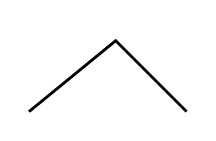
\begin{tikzpicture}[scale=1]
		\draw[-,line width=1pt] (0,0) -- (1.1,0.9) -- (2,0);
		\SetVertexSimple[Shape=circle,FillColor=white,MinSize=8 pt]
		\Vertex[x=0.00, y=0]{a}
		\Vertex[x=-0.5, y=1]{b}
		\Vertex[x=2., y=0]{c}
		\Edges(a,b,c)
		\tikzstyle{vertex}=[circle,minimum size=5pt]
		\node[vertex] (v0) at (1.1,0.9) {};
		\Edges(a,v0,c)
		
		%\node[vertex] (v1) at (-0.5,1) {b};
		%\node[vertex] (v2) at (2,0) {c};
		\end{tikzpicture} 
		\\
		&(a)&&(b)
	\end{tabular}
\end{center}
	\caption{Dibujos de $K_3$} \label{fA4.1}
\end{figure}

Pero la definición es que un grafo es planar si se {\em puede}
dibujar en el plano sin cruces de aristas, no si {\em todo} dibujo
no tiene cruces. (Si la definición fuera así, ningún grafo seria
planar, pues siempre se puede dibujar cualquier grafo con cruces).
Otro ejemplo, ya visto, $K_4$ puede ser dibujado como en la Fig. \ref{fA4.2}-(a) 
y no parece planar, pero dibujado como en la Fig. \ref{fA4.2}-(b) muestra que $K_4$ es planar.

\begin{figure}[ht]
	\begin{center}
	\begin{tabular}{cccc}
		&
		\begin{tikzpicture}[scale=1]
		\SetVertexSimple[Shape=circle,FillColor=white,MinSize=8 pt]
		\Vertex[x=0.00, y=0]{a}
		\Vertex[x=2, y=0]{b}
		\Vertex[x=2, y=2]{c}
		\Vertex[x=0, y=2]{d}
		\Edges(a,b,c,d,a)
		\Edges(a,c)
		\Edges(b,d)
		\end{tikzpicture}
		&
		\qquad
		& 
		\begin{tikzpicture}[scale=1]
				\SetVertexSimple[Shape=circle,FillColor=white,MinSize=8 pt]
		\Vertex[x=0.00, y=0]{a}
		\Vertex[x=1.15, y=2]{b}
		\Vertex[x=2.31, y=0]{c}
		\Vertex[x=1.15, y=0.8]{d}
		\Edges(a,b,c,d,a)
		\Edges(a,c)
		\Edges(b,d)
		\end{tikzpicture} 
		\\
		&(a)&&(b)
	\end{tabular}
\end{center}
	\caption{Dibujos de $K_4$} \label{fA4.2}
\end{figure}

En vista de estos ejemplos, una pregunta es ?`existen grafos no
planares? Por ejemplo si dibujáramos $K_{16}$ parecería imposible
que fuera planar, dada la gran cantidad de cortes, pero ?`cómo
podemos estar seguros?

Observemos primero que si $G$ es planar y $H$ es subgrafo de $G$,
entonces $H$ es planar, pues, si podemos dibujar a $G$ en el plano
sin cortes de aristas, entonces $H$ que esta ``metido'' en $G$,
también puede ser así dibujado. Así, como ya vimos que $K_4$ es
planar, sabemos que todo subgrafo de él es planar; es decir, todo
grafo con cuatro o menos vértices es planar. Esta observación
tiene consecuencias en la otra dirección también: si encontramos
un grafo $H$ que {\em no} sea planar, entonces todo grafo $G$ que
lo tenga como subgrafo deberá necesariamente ser no planar, pues
si $G$ fuera planar, $H$ también lo seria. Así, si queremos probar
que $K_{16}$ no es planar, bastará con encontrar algún subgrafo
mas sencillo de el que no lo sea. De hecho, probaremos que $K_5$
no es planar, con lo cual todos los grafos $K_n$, con $n\ge 5$ son
no planares.

En lo que sigue veremos un arma poderosa para probar que un grafo
es no planar: la llamada ``fórmula de Euler''.
 \index{fórmula de Euler}
Supongamos que un grafo {\em sí} es planar. Escojamos un diagrama
de él en el plano (puede haber muchos, escojamos uno). Este
diagrama divide al plano en varias regiones. Por ejemplo, si $G$
esta representado por el dibujo de la Fig. \ref{fA4.3}, entonces
se obtienen regiones que numeraremos como en la Fig. \ref{fA4.4}
($1$ es la región ``exterior'' a todo el grafo).

\begin{figure}[h]
	\begin{center}
\begin{tikzpicture}[scale=0.7]
\SetVertexSimple[Shape=circle,FillColor=white,MinSize=8 pt]
\Vertex[x=0.00, y=0]{0}
\Vertex[x=0.5, y=2]{1}
\Vertex[x=0.8, y=-2]{2}
\Vertex[x=1.5, y=-0.2]{3}
\Vertex[x=1.8, y=-2.2]{4}
\Vertex[x=3.5, y=1.9]{5}
\Vertex[x=3, y=0.1]{6}
\Vertex[x=3.7, y=-1.7]{7}
\Vertex[x=4, y=-0.1]{8}
\Vertex[x=6, y=0.3]{9}
\Vertex[x=5.5, y=1.8]{10}
\Vertex[x=6, y=-2.2]{11}
\Vertex[x=6.8, y=2]{12}
\Vertex[x=7, y=-1.8]{13}
\Vertex[x=7.5, y=0.8]{14}
\Vertex[x=8.5, y=1.8]{15}
\Vertex[x=9, y=-1]{16}
\Edges(0,1,3,4,2,0)
\Edges(1,5,6,7,4,7,8,5,9,8,9,7,11,9,5,10,12,14,15,16,13,11)
\end{tikzpicture} 
\end{center}
\caption{Un grafo planar} \label{fA4.3}
\end{figure}

En realidad, también podríamos considerar a la región formada por
las regiones $3$ y $4$ juntas, o $2$, $5$ y $6$ juntas, etc. Pero nuestra
preocupación estará centrada en una de estas regiones ``simples'',
a las cuales llamaremos {\em caras}.
 \index{caras de un grafo planar}


\begin{figure}[h]
	\begin{center}
	\begin{tikzpicture}[scale=0.7]
	\SetVertexSimple[Shape=circle,FillColor=white,MinSize=8 pt]
	\Vertex[x=0.00, y=0]{0}
	\Vertex[x=0.5, y=2]{1}
	\Vertex[x=0.8, y=-2]{2}
	\Vertex[x=1.5, y=-0.2]{3}
	\Vertex[x=1.8, y=-2.2]{4}
	\Vertex[x=3.5, y=1.9]{5}
	\Vertex[x=3, y=0.1]{6}
	\Vertex[x=3.7, y=-1.7]{7}
	\Vertex[x=4, y=-0.1]{8}
	\Vertex[x=6, y=0.3]{9}
	\Vertex[x=5.5, y=1.8]{10}
	\Vertex[x=6, y=-2.2]{11}
	\Vertex[x=6.8, y=2]{12}
	\Vertex[x=7, y=-1.8]{13}
	\Vertex[x=7.5, y=0.8]{14}
	\Vertex[x=8.5, y=1.8]{15}
	\Vertex[x=9, y=-1]{16}
	\Edges(0,1,3,4,2,0)
	\Edges(1,5,6,7,4,7,8,5,9,8,9,7,11,9,5,10,12,14,15,16,13,11)
	\draw (-2, 1) node {1};
	\draw (3.5, 0) node {2};
	\draw (4.3, 0.8) node {3};
	\draw (4.3, -0.7) node {4};
	\draw (2.2, 0) node {5};
	\draw (0.8, 0) node {6};
	\draw (5.4, -1.2) node {7};
	\draw (7.2, -0.5) node {8};
	\end{tikzpicture} 
	\end{center}
	\caption{Regiones de un grafo planar} \label{fA4.4}
\end{figure}


Observemos que no podemos hablar propiamente de las caras del
grafo (aunque a veces lo haremos así) pues ellas son en realidad
dependientes del diagrama, no del grafo. Sin embargo, algo puede
decirse acerca de ellas:

\begin{teorema}\label{tA4.1} (Fórmula de Euler) Sea $G$ un grafo
conexo, con $v$ vértices, y $e$ aristas. Supongamos que en algún
diagrama planar de $G$, existen $f$ caras. Entonces, $v-e+f=2$.
\end{teorema}

Antes de ver la prueba, observemos que, puesto que $v$ y $e$
dependen de $G$ y no del diagrama, la fórmula de Euler dice que no
importa como dibujemos a $G$ en el plano (siempre y cuando esto
sea posible), entonces siempre obtendremos $e-v+2$ caras. Por lo
tanto, el {\it número} de caras es algo independiente del
diagrama, y podemos hablar del ``número de caras de un grafo
planar''. Otra observación es que en el número de caras estamos
contando la cara infinita, es decir, la exterior a todo el grafo.
Finalmente, observemos que se pide que $G$ sea conexo. La fórmula
debe ser alterada en caso contrario.



\begin{proof}[Demostración del teorema \ref{tA4.1}]
Supongamos que la fórmula de Euler no sea cierta. Es decir,
supongamos que existen grafos planares para los cuales la fórmula
no es válida. Tomemos, de todos estos contraejemplos, alguno con
$e$ tan chico como sea posible, y llamemos $G$ a ese grafo.
Observemos que $G$ debe tener por lo menos un ciclo, pues si fuera
acíclico, como es conexo, sería un árbol. Ahora bien, en un árbol,
$e=v-1$. Además, por ser acíclico, no hay caras, salvo la cara
infinita, es decir, $f$ seria 1. Pero entonces
$v-e+f=v-(v-1)+1=v-v+1+1=2$ y $G$ no sería un contraejemplo. Así
pues, $G$ tiene al menos un ciclo. Sea $xy$ alguna arista
perteneciente a algún ciclo, y consideremos $H=G-xy$. Como $xy$
pertenece a algún ciclo, es una arista que separa dos caras en
$G$. Esas dos caras ahora son una sola en $H$. 
Ver Fig. \ref{fA4.5}.


\begin{figure}[ht]
	\begin{center}
	\begin{tabular}{cccc}
		&
		\begin{tikzpicture}[scale=0.7]
		\SetVertexSimple[Shape=circle,FillColor=white,MinSize=8 pt]
		\Vertex[x=0.00, y=0]{0}
		\Vertex[x=0.5, y=-1]{1}
		\Vertex[x=-0.5, y=-2]{2}
		\Vertex[x=0, y=-3]{3}
		\Vertex[x=2, y=-4]{4}
		\Vertex[x=3.5, y=-3]{5}
		\Vertex[x=3.5, y=-2]{6}
		\draw (3., -2.1) node {$y$};
		\Vertex[x=2, y=-1]{7}
		\draw (2, -1.5) node {$x$};
		\Vertex[x=1.8, y=0.2]{8}
		\Vertex[x=3, y=0]{9}
		\Vertex[x=5, y=-0.2]{10}
		\Vertex[x=4.5, y=-2.7]{11}
		\Edges(0,1,2,3,4,5,6)
		\Edges(6,7)
		\Edges(7,8,0)
		\Edges(1,7)
		\Edges(8,9,10,11,5)
		\draw (1.5, -2.5) node {$A$};
		\draw (3.5, -1) node {$B$};
		\end{tikzpicture}
		&
		\qquad
		& 
		\begin{tikzpicture}[scale=0.7]
		\SetVertexSimple[Shape=circle,FillColor=white,MinSize=8 pt]
		\Vertex[x=0.00, y=0]{0}
		\Vertex[x=0.5, y=-1]{1}
		\Vertex[x=-0.5, y=-2]{2}
		\Vertex[x=0, y=-3]{3}
		\Vertex[x=2, y=-4]{4}
		\Vertex[x=3.5, y=-3]{5}
		\Vertex[x=3.5, y=-2]{6}
		\draw (3., -2.1) node {$y$};
		\Vertex[x=2, y=-1]{7}
		\draw (2, -1.5) node {$x$};
		\Vertex[x=1.8, y=0.2]{8}
		\Vertex[x=3, y=0]{9}
		\Vertex[x=5, y=-0.2]{10}
		\Vertex[x=4.5, y=-2.7]{11}
		\Edges(0,1,2,3,4,5,6)
		\Edges(7,8,0)
		\Edges(1,7)
		\Edges(8,9,10,11,5)
		\end{tikzpicture} 
	\end{tabular}
\end{center}
	\caption{Eliminar una arista} \label{fA4.5}
\end{figure}
Así, si $f_H,e_H$ y $v_H$ denotan el número de caras, aristas y
vértices de $H$ respectivamente, te\-ne\-mos que $f_H=f-1$. Además,
como borramos una arista, $e_H=e-1$, y como el número de vértices
no cambia, $v_H=v$.

Pero, $e_H=e-1$ es menor que $e$, y $G$ era un contraejemplo con
un número tan chico como fuera posible de aristas, por lo tanto,
$H$ no es un contraejemplo, es decir, $v_H-e_H+f_H=2$.
Reemplazando, obtenemos:
$$
v-e+f=v_H-(e_H+1)+f_H+1=v_H-e_H-1+f_H+1=v_H-e_H+f_H=2,
$$
lo cual dice que $G$ no es un contraejemplo, absurdo.
\end{proof}

La fórmula de Euler es una herramienta muy poderosa en la teoría
de grafos planares. Para empezar, permite probar que un grafo
planar no puede tener muchas aristas, en relación a sus vértices

\begin{corolario}\label{cA4.1} Sea $G$ un grafo planar con al menos $3$
vértices. Entonces, $e\le 3v-6$, donde $e$ es el número de aristas
y $v$ el número de vértices de $G$.
\end{corolario}
\begin{proof} Consideremos las caras de $G$. Si es una cara
distinta de la cara infinita, es porque viene de un ciclo. Ahora
bien, todo ciclo debe tener por lo menos $3$ aristas, así que
podemos concluir que hay por lo menos $3$ aristas en el borde de esa
cara. Si, en cambio, es la cara infinita y el grafo tiene más de
tres aristas entonces ``toca'' $3$ o más aristas. Si el grafo tiene
menos de $3$ aristas (y ningún ciclo), es uno de los de la Fig. \ref{fA4.6}. 
Como estamos suponiendo que hay al menos $3$ vértices,
en realidad solo hay que considerar el último caso, y ese tiene
$e=2$, $v=3$, y $2\le 3 \cdot 3-6$.

\begin{figure}[ht]
	\begin{center}
	\begin{tabular}{cccc}
		&
		\begin{tikzpicture}[scale=0.7]
		\SetVertexSimple[Shape=circle,FillColor=white,MinSize=8 pt]
		\Vertex[x=0.00, y=0]{0}
		\Vertex[x=2, y=0]{1}
		\Edges(0,1)
		\end{tikzpicture}
		&
		\qquad\qquad
		& 
		\begin{tikzpicture}[scale=0.7]
		\SetVertexSimple[Shape=circle,FillColor=white,MinSize=8 pt]
		\Vertex[x=0.00, y=0]{0}
		\Vertex[x=2, y=0]{1}
		\Vertex[x=4, y=0]{2}
		\Edges(0,1,2)
		\end{tikzpicture} 
	\end{tabular}
\end{center}
	\caption{Grafos acíclicos con menos de 3 aristas} \label{fA4.6}
\end{figure}


Así pues, podemos suponer que en nuestro grafo, todas las caras
tienen al menos $3$ aristas en su borde. Es decir:
$$
\begin{aligned}
3\le &\,\text{\rm Número de aristas en el borde de cara }1 \\
3\le &\,\text{\rm Número de aristas en el borde de cara }2\\
&\vdots \\
3\le &\,\text{\rm Número de aristas en el borde de cara }f.
\end{aligned}
$$
Si sumamos estas desigualdades, del lado izquierdo obtendremos
$3f$. En el lado derecho, cada arista puede, o bordear dos caras,
o bordear una. Pero ciertamente, no puede haber aristas que sean
borde de $3$ caras. Así, si sumamos en el lado izquierdo, la suma
nos dará menor o igual a $2e$. Por lo tanto, $3f\le 2e$. Tomando
la fórmula de Euler y multiplicándola por $3$, obtenemos:
$3v-3e+3f=6$. Usando ahora $3f\le 2e$, tenemos
$$
6=3v-3e+3f\le 3v-3e+2e=3v-e,$$ es decir, $e\le 3v-6$.
\end{proof}

Este corolario nos permite probar inmediatamente la no planaridad
de un número significativo de grafos. Por ejemplo, recordemos que
queríamos ver que $K_5$ era no planar. Esto lo obtenemos en forma
directa, pues $K_5$ tiene $5$ vértices y $10$ aristas, por lo tanto,
si fuera planar debiéramos tener que $10\le 3\cdot 5-6=15-6=9$, lo cual
no es cierto.
\end{section}




\begin{section}{El problema del agua-luz-gas}\label{Ap4.2}
Este es un conocido problema de escuela primaria: existen tres
casas, y tres centrales: la del agua, la de la luz y la del gas.
Trazar las cañerías desde las centrales a las casas sin que se
crucen. Una solución (pero haciendo trampa) es mandar las tres
cañerías a una casa, y de ella sacarlas las tres a la otra, y de
ella las tres a la otra:

\begin{figure}[ht]
	\begin{center}
	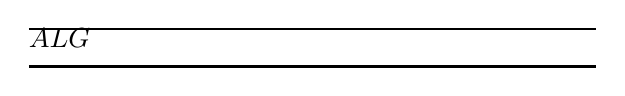
\begin{tikzpicture}[scale=1.2]
	\draw[-,line width=0.8pt] (0,0.2) -- (3,0.2) -- (6,0.2);
	\draw[-,line width=0.8pt] (0,-0.2) -- (3,-0.2) -- (6,-0.2);
	{\renewcommand{\VertexShape}{rectangle}
	\Vertex[x=0.00, y=0, L=Primera casa]{0}
	\Vertex[x=3, y=0, L=Segunda casa]{1}
	\Vertex[x=6, y=0, L=Tercera casa]{2}
	\Vertex[x=0.00, y=-2, L=$A$]{3}
	\Vertex[x=3, y=-2, L=$L$]{4}
	\Vertex[x=6, y=-2, L=$G$]{5}
	}
	\SetVertexSimple[Shape=rectangle,FillColor=white,MinSize=8 pt]
	%\draw (0, 0) node {$\boxed{\text{Primera casa}}$};
	\Edges(0,1,2)
	\Edges(3,0)
	\Edges(4,0)
	\Edges(5,0)
	
	\end{tikzpicture}
	\end{center}
	\caption{Una solución tramposa} \label{fA4.7}
\end{figure}

En realidad, no permitiremos el uso de intermediarios, es decir el
problema será llevar directamente la cañería desde cada central a
cada casa. En el lenguaje de la teoría de grafos, consiste en
representar, en el plano, al grafo $K_{3,3}$ Fig. \ref{fA4.8}.


\begin{figure}[ht]
	\begin{center}
	\begin{tikzpicture}[scale=1.2]
	{\renewcommand{\VertexShape}{rectangle}
		\Vertex[x=0.00, y=0, L=Primera casa]{0}
		\Vertex[x=3, y=0, L=Segunda casa]{1}
		\Vertex[x=6, y=0, L=Tercera casa]{2}
		\Vertex[x=0.00, y=-2, L=$A$]{3}
		\Vertex[x=3, y=-2, L=$L$]{4}
		\Vertex[x=6, y=-2, L=$G$]{5}
	}
	\Edges(0,4)
	\Edges(0,5)
	\Edges(1,3)\Edges(1,4)
	\Edges(1,5)
	\Edges(2,3)\Edges(2,4)
	\Edges(2,5)
	\Edges(3,0)
	\Edges(4,0)
	\Edges(5,0)
	
	\end{tikzpicture}
	\end{center}
	\caption{Luz-agua-gas es $K_{3,3}$} \label{fA4.8}
\end{figure}

La pregunta es entonces si $K_{3,3}$ es planar o no. Veamos si
podemos usar esta fórmula que probamos recién: $K_{3,3}$ tiene $9$
aristas, y $6$ vértices. Desafortunadamente, $3 \cdot 6-6=18-6=12$ es
ciertamente mayor que $9$, así que solo sabemos que quizás es
planar. Pero, observemos que $K_{3,3}$, por ser bipartito, no
tiene ningún triángulo como subgrafo. Así pues, deduciremos la no
planaridad de $K_{3,3}$ del si\-guien\-te

\begin{corolario}\label{cA4.2} Si $G$ es un grafo planar con por lo menos $3$ vértices y que no tiene ningún triángulo como subgrafo, entonces
$e\le 2v-4$.
\end{corolario}
\begin{proof} Es similar a la demostración del corolario \ref{cA4.1}, pero como no hay
triángulos, todo ciclo tiene por lo menos $4$ aristas, es decir,
cada cara esta bordeada por al menos $4$ aristas. Las únicas
excepciones con al menos $3$ vértices son:



\begin{figure}[ht]
	\begin{center}
	\begin{tabular}{cccccc}
	&
	\begin{tikzpicture}[scale=0.5]
	\SetVertexSimple[Shape=circle,FillColor=white,MinSize=8 pt]
	\Vertex[x=0.00, y=0]{0}
	\Vertex[x=2, y=0]{1}
	\Vertex[x=4, y=0]{2}
	\Edges(0,1,2)
	\end{tikzpicture}
	&
	\qquad
	& 
	\begin{tikzpicture}[scale=0.5]
	\SetVertexSimple[Shape=circle,FillColor=white,MinSize=8 pt]
	\Vertex[x=0.00, y=0]{0}
	\Vertex[x=2, y=0]{1}
	\Vertex[x=4, y=0]{2}
	\Vertex[x=6, y=0]{3}
	\Edges(0,1,2,3)
	\end{tikzpicture} 
	&
	\qquad
	&
	\begin{tikzpicture}[scale=0.5]
	\SetVertexSimple[Shape=circle,FillColor=white,MinSize=8 pt]
	\Vertex[x=0.00, y=0]{0}
	\Vertex[x=0, y=1.3]{1}
	\Vertex[x=-1, y=-1]{2}
	\Vertex[x=1, y=-1]{3}
	\Edges(0,1,0,2,0,3)
	\end{tikzpicture} 
	\end{tabular}
\end{center}
	\caption{Grafos acíclicos con menos de $4$ aristas y al menos $3$
	vértices} \label{fA4.9}
\end{figure}

En el primer caso, $e=2$, $v=3$ y $2 \cdot 3-4=6-4=2$. En el segundo y
terceros, $e=3$, $v=4$ y $2 \cdot 4-4=8-4=4\ge 3$. Así pues, podemos
suponer que cada cara esta bordeada por al menos $4$ aristas.
Sumando cara a cara, como antes, obtenemos ahora $4f\le 2e$, es
decir, $2f\le e$. Multiplicando la fórmula de Euler por $2$,
tenemos: $4=2v-2e+2f\le 2v-2e+e=2v-e$, es decir, $e\le 2v-4$.
\end{proof}

Retornando a $K_{3,3}$, como no tiene triángulos, podemos aplicar
este corolario, y si fuera planar, debería cumplirlo. Pero
habíamos dicho que $K_{3,3}$ tiene $9$ aristas y $6$ vértices, y
$2\cdot 6-4=12-4=8$. Por lo tanto, $K_{3,3}$ no es planar.

Una ultima observación acerca de grafos planares: existe un
teorema muy interesante, de difícil demostración (la prueba tiene
$31$ casos y subcasos para considerar) debido a Kuratowski, que
 \index{Teorema de Kuratowski}
 dice que $K_5$ y $K_{3,3}$ son los dos grafos
``básicos'' no planares, en el siguiente sentido: un grafo $G$ es
no planar si y solo si existe un subgrafo de $G$, digamos $H$, tal
que $H$ se ``ve'' como $K_5$ o como $K_{3,3}$, es decir, $H$ es
uno de ellos, excepto que tal vez, ``agregue'' en alguna o algunas
aristas, vértices en el medio. Por ejemplo, $H$ puede lucir como


\begin{figure}[ht]
	\begin{center}
	\begin{tikzpicture}[scale=1]
	\SetVertexSimple[Shape=circle,MinSize=5 pt,FillColor=white]
	\Vertex[x=0.00, y=2.00]{1}
	\Vertex[x=1.90, y=0.62]{2}
	\Vertex[x=1.18, y=-1.62]{3}
	\Vertex[x=-1.18, y=-1.62]{4}
	\Vertex[x=-1.90, y=0.62]{5}
	\Edges(1,2,3,4,5,1)
	\Edges(1,3,5,2,4,1)
	\Vertex[x=0.95, y=1.31]{a}
	\Vertex[x=0.3, y=1.08]{b}
	\Vertex[x=1.54, y=-0.5]{c}
	\Vertex[x=-0.36, y=-0.5]{d}
	\Vertex[x=-0.95, y=1.31]{e}
	\Vertex[x=-0.39, y=-1.62]{f}
	\Vertex[x=0.39, y=-1.62]{g}
	\end{tikzpicture}
	\end{center}
	\caption{}\label{fA4.10}
\end{figure}


\end{section}





\begin{section}{El teorema de los cuatro colores} \label{Ap4.3}

Juntaremos ahora lo que hemos visto en esta sección con lo que
vimos en la anterior, para tratar uno de los problemas mas famosos
y recalcitrantes de la teoría de grafos, a saber: ?`cuántos
colores se necesitan para colorear un grafo planar? En otras
palabras, si quiero estar seguro de poder colorear propiamente los
vértices de cualquier grafo planar, ?`cuántos colores necesito
tener? De hecho, una pregunta más básica sería si existe una
cantidad finita de colores que me permitan colorear cualquier tipo
de grafo planar, por grande que sea. (Es claro que la respuesta
para grafos en general es negativa, pues $K_n$ requiere $n$
colores.) Como $K_4$ es planar, sabemos que necesitamos por lo
menos $4$ colores. No podemos decir que necesitamos necesariamente
$5$, pues hemos visto que $K_5$ no es planar. Pero, podría haber
otro grafo, complicado pero planar, que requiera $5$, o más,
colores. A mediados del siglo pasado la conjetura de que bastan $4$
colores fue hecha, y en $1\,879$ A. Kempe publicó una prueba de este
hecho, que paso a llamarse el teorema de los cuatro colores.
Desafortunadamente para Kempe, en $1\,889$ (diez años después) otro
matemático, P. Heawood, probó que la prueba de Kempe contenía un
error. Heawood no fue completamente destructivo: mostró que
adaptando la prueba de Kempe, podía probarse que con $5$ colores
bastaba para colorear cualquier grafo planar (el teorema de los
cinco colores). Así pues, quedo planteado el problema de saber si
el teorema de los cuatro colores era cierto, o bien si existía
algún grafo planar para el cual $5$ colores fueran necesarios.
(Pero, al menos, gracias a Heawood, no era necesario buscar alguno
que necesitara $6$, o $7$ u $8$ colores, pues no existen, gracias al
teorema de los cinco colores.) De hecho, en ese mismo artículo,
Heawood probó más cosas: existe algo llamado género de un grafo,
que es un número entero no negativo. Heawood demostró que existía
una \index{género de un grafo} fórmula (expresión aritmética) que
para cada género $g\ge 1$ da la cantidad de colores que permite
colorear todos los grafos de género $g$. Los grafos planares tiene
género igual a $0$ y aplicando la fórmula para $g=0$ obtenemos el
número $4$. Sin embargo, Heawood pudo probar que la fórmula es
válida si $g$ es mayor o igual a 1. El hecho de que esta fórmula
existiera ``convenció'' a mucha gente de que el teorema de los
cuatro colores debía ser cierto y que una prueba no tardaría en
hallarse. Sin embargo, pese al esfuerzo de muchos matemáticos y
pese al desarrollo de la teoría, el teorema de los cuatro colores
no pudo probarse hasta $1975$, cuando dos matemáticos \index{Teorema
de los cuatro colores} norteamericanos, K. Appel y W. Haken, lo
probaron. Más aún, no pudieron probarlos solos, sino que debieron
usar la ``ayuda'' de un poderoso (para esa época) computador. Así,
aún cuando el teorema fue probado, un gran sentimiento de
desconfianza se generó, sobretodo en una época en la cual el
acceso fácil a tiempo de computador no era común. Veinte años han
pasado y la prueba ahora ha sido controlada numerosas veces y no
genera tanta resistencia como antes. Aún así, si alguien pudiese
publicar una prueba que fuese ``leíble por humanos'' sería muy
bien bienvenido.

Obviamente por lo dicho arriba, no daremos una prueba del teorema
de los cuatro colores. Sí daremos una del teorema de los cinco
colores\index{Teorema de los cinco colores}, mencionando donde se encuentra la dificultad de la demostración del teorema de los  cuatro colores, y dando una idea de
que es lo que Appel y Haken (y el computador) hicieron.

\begin{lema} \label{lA4.3.1} Sea $G$ un grafo planar. Entonces, existe
un vértice de $G$ de valencia $5$ o menos.
\end{lema}
\begin{proof} Si el orden de $G$ es menor o igual a $2$, esto
es obvio, pues la valencia de cualquier vértice no superará $2$.
Así, podemos suponer que hay al menos $3$ vértices, y por lo tanto,
sabemos que $e\le 3v-6$, donde $e$ es el numero de aristas y $v$
el de vértices.

Supongamos ahora que la valencia de todos los vértices sea al
menos $6$. Entonces, si sumamos las valencias de todos los vértices,
la suma sera mayor o igual a $6v$. Pero la suma de todos las
valencias es igual a $2e$ (lema del apretón de manos). Así,
tenemos que $2e\ge 6v$. Por otro lado, como $e\le 3v-6$, tenemos
que $2e\le 6v-12$, es decir, obtenemos $6v-12\ge 2e\ge 6v$, o
$-12\ge 0$, lo cual es un absurdo.
\end{proof}

\begin{teorema}\label{tA4.3.1}(Teorema de los cinco colores) Si $G$ es
planar, $\chi (G)\le 5$.
\end{teorema}
\begin{proof}
 Supongamos que no sea cierto. De todos los
contraejemplos al teorema, escojamos uno con la menor cantidad de
vértices posible y llamémosle $G$. Por el lema anterior, existe un
vértice $x$ de $G$ con valencia menor o igual a 5. Consideremos
$H=G-\{x\}$, que es un grafo con menos vértices que $G$ y por lo tanto
no puede ser un contraejemplo; es decir, $\chi (H)\le 5$. Así,
podemos colorear $H$ con 5 colores. Si la valencia de $x$ en $G$
es $0,1,2,3$ o $4$, los vértices adyacentes a $x$ ``usan'' a lo sumo
$4$ de los $5$ colores, así que podemos colorear a $x$ con el quinto
color, y tendríamos que $\chi (G)=5$, lo cual no es posible pues
$G$ es un contraejemplo. Así pues, podemos suponer que la valencia
de $x$ es $5$. Ahora bien, si los cinco vértices adyacentes a $x$ no
usan cinco colores, estamos como antes, y podemos colorear a $x$
con el color faltante. Así, no solo podemos suponer que hay cinco
vértices adyacentes a $x$, sino también que cada uno esta
coloreado con un color distinto. Llamemos a estos vértices
$y,z,u,w,t$, y supongamos que $y$ de color $1$, $z$ de color dos,
etc.

\begin{figure}[h]
	\begin{center}
\begin{tikzpicture}[scale=0.5]
\SetVertexSimple[Shape=circle,FillColor=white,MinSize=8 pt]
\Vertex[x=0.00, y=0]{0}
\Vertex[x=0.5, y=2]{1}
\Vertex[x=4, y=1.5]{2}
\Vertex[x=3, y=-1.4]{3}
\Vertex[x=0.5, y=-2]{4}
\Vertex[x=-3, y=0]{5}
\draw (-0.5, 0.4) node {$x$};
\draw (-0.1, 2) node {$y$};
\draw (1.4, 2) node {$(1)$};
\draw (3.4, 1.7) node {$z$};
\draw (4.8, 1.7) node {$(2)$};
\draw (2.4, -1.6) node {$u$};
\draw (3.8, -1.6) node {$(3)$};
\draw (-0.2, -2) node {$w$};
\draw (1.3, -2) node {$(4)$};
\draw (-3.4,0.5) node {$t$};
\draw (-2.3, 0.5) node {$(5)$};
\Edges(0,1,0,2,0,3,0,4,0,5)
\end{tikzpicture} 
\end{center}
\caption{}\label{fA4.11}
\end{figure}

Supongamos primero que no haya, entre $y$ y $u$, ningún camino tal
que el color de todos sus vértices sea $1$ o $3$. Entonces, podemos
cambiarle el color a $y$, de color $1$ a color $3$. Además, a los
vértices adyacentes a $y$ que tengan color $3$, les cambiamos el
color de $3$ a $1$. A los vértices adyacentes a estos, que tengan
color $1$, los cambiamos a $3$, y así sucesivamente. Después de
realizar todos estos cambios, todavía tenemos un coloreo propio.
Ahora bien, como estamos suponiendo que no hay ningún camino de
color $1$ y $3$ exclusivamente entre $y$ y $u$, resulta que $u$ no
cambia de color, es decir, retiene el color $3$. Pero $y$ ahora
tiene también el color $3$, y ningún otro vértice adyacente a $x$
tiene el color $1$. Pero, entonces, podemos colorear a $x$ con el
color $1$ sin problemas, absurdo pues $\chi(G)\ge 6$.

Así pues, existe un camino con todos los vértices de color $1$ y $3$
entre $y$ y $u$. Igualmente, si no hubiera ningún camino con todos
los vértices de color $2$ y $4$ entre $z$ y $w$, le podemos cambiar el
color a $z$ de $2$ a $4$ sin problemas, y colorear a $x$ con el color
$2$. Así, también podemos suponer que existe un camino con todos los
vértices de color $2$ y $4$ entre $z$ y $w$.


\begin{figure}[h]
	\begin{center}
	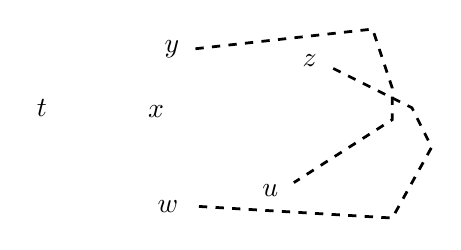
\begin{tikzpicture}[scale=0.5]
	\draw[-,line width=1pt,dashed] (0.5,2) -- (5,2.5) -- (5.5,1)-- (5.5,0.2) -- (3, -1.4) ;
	\draw[-,line width=1pt,dashed] (4,1.5) -- (6,0.5) -- (6.5,-0.5)-- (5.5,-2.3) -- (0.5, -2) ;
	\SetVertexSimple[Shape=circle,FillColor=white,MinSize=8 pt]
	\Vertex[x=0.00, y=0]{0}
	\Vertex[x=0.5, y=2]{1}
	\Vertex[x=4, y=1.5]{2}
	\Vertex[x=3, y=-1.4]{3}
	\Vertex[x=0.5, y=-2]{4}
	\Vertex[x=-3, y=0]{5}
	\draw (-0.5, 0.4) node {$x$};
	\draw (-0.1, 2) node {$y$};
	\draw (3.4, 1.7) node {$z$};
	\draw (2.4, -1.6) node {$u$};
	\draw (-0.2, -2) node {$w$};
	\draw (-3.4,0.5) node {$t$};
	\Edges(0,1,0,2,0,3,0,4,0,5)
	\end{tikzpicture} 
	\end{center}
	\caption{Caminos de $y$ a $u$ y de $z$ a $w$} \label{fA4.12}
\end{figure}


Por la Fig. \ref{fA4.12} es claro que tenemos un problema: ?`por
donde se cruzan los caminos $A$ y $ B$? Más precisamente, el
camino $A$, junto con las aristas $xy$ y $xu$, forma un ciclo $C$.
Este ciclo tiene un interior y un exterior. El ciclo $ D$ formado
por $B$ y las aristas $xz$, $xw$ cruza al ciclo $C$ en el punto
$x$, pues la arista $xz$ esta en el interior y la arista $xw$ en
el exterior de $C$. Por lo tanto, $D$ debe cruzar a $C$ en algún
otro punto. Pero no puede hacerlo, pues en el resto, $C$ esta
coloreado con los colores $1$ y $3$, y $D$ con los colores $2$ y $4$.
Hemos llegado a una contradicción.
\end{proof}

Analicemos un poco la prueba: hemos probado dos cosas:\\
\noindent (1) todo grafo planar debe tener una de las siguientes ``configuraciones'',
es decir, parte de él debe lucir como alguno de los grafos de la
Fig. \ref{fA4.13}.


\begin{figure}[h]
	\begin{center}
	\begin{tikzpicture}[scale=0.5]
	\SetVertexSimple[Shape=circle,FillColor=white,MinSize=8 pt]
	\Vertex[x=0.00, y=0]{0}
	\Vertex[x=3, y=0]{1}
	\Vertex[x=5, y=0]{2}
	\Vertex[x=7, y=1]{3}
	\Vertex[x=9, y=-1]{4}
	\Vertex[x=11, y=1]{5}
	\Vertex[x=13, y=1]{6}
	\Vertex[x=15, y=-1]{7}
	\Vertex[x=17, y=1]{8}
	\Vertex[x=15, y=-3]{9}
	\Edges(1,2)
	\Edges(3,4,5)
	\Edges(6,7,8,7,9)
	\Vertex[x=0, y=-3]{a}
	\Vertex[x=4, y=-3]{b}
	\Vertex[x=0, y=-7]{c}
	\Vertex[x=4, y=-7]{d}
	\Edges(a,d)
	\Edges(b,c)
	\Vertex[x=2, y=-5]{e}
	\Vertex[x=7, y=-4]{f}
	\Vertex[x=11, y=-4]{g}
	\Vertex[x=9, y=-5.5]{h}
	\Vertex[x=9, y=-3]{i}
	\Vertex[x=7, y=-7]{j}
	\Vertex[x=11, y=-7]{k}
	\Edges(f,h,g,h,i,h,j,h,k)
	\end{tikzpicture} 
	\end{center}
\caption{Posibles configuraciones} \label{fA4.13}
\end{figure}


Esto lo probamos con el lema \ref{lA4.3.1}. Es decir, probamos que
ese conjunto de configuraciones es lo que se llama {\it inevitable}.


Además, probamos que si un grafo planar tiene una de esas
configuraciones, puede ser coloreado con $5$ colores (esto es lo que
hicimos en el teorema). Es decir, probamos que ese conjunto de
con\-fi\-gu\-ra\-cio\-nes es lo que se llama {\it irreducible} (para $5$
colores). Kempe creyó que había sido capaz de probar que todo
grafo planar que tuviera esas configuraciones podía ser coloreado
con $4$ colores, y muchos autores después de Heawood trataron de
probar lo mismo. Pero luego se descubrieron nuevas técnicas, tanto
para probar que un conjunto de configuraciones es irreducible,
como para probar que es inevitable. Lo que no se podía hacer era
encontrar un conjunto que fuera al mismo tiempo irre\-du\-ci\-ble (para
$4$ colores) e inevitable. Finalmente, Appel y Haken encontraron un
conjunto que satisfacía esas propiedades. Solo que en vez detener
$6$ elementos, como en el caso del teorema de $5$ colores, el conjunto
de Appel y Haken tiene $1\,480$ elementos, y ningún ser humano es
capaz de probarlo, sino que es necesario un computador para
comprobar la inevitabilidad e irreducibilidad.


\end{section}

